% /* GRASP: Copyright 1997,1998  Bruce Allen */
% $Id: man_binary-search.tex,v 1.21 1999/07/11 21:22:09 ballen Exp $
\section{Binary Inspiral Search on November 1994 Data}
\label{s:binary-search}
\setcounter{equation}0
This section includes and documents the code that was used to perform
a binary inspiral search of the Caltech 40-meter data from November
1994.
The goal of this work was to place an upper limit on the event
rate for binary inspiral in our galaxy.  This section includes the
following items:
\begin{itemize}
\item
Source code for the search.
\item
Source code for generating simulated signals with ``galactic''
distribution.
\item
Scripts for running the code on a Beowulf-type system (see\\
\htmladdnormallink{{\tt www.lsc-group/phys.uwm.edu/$\sim$www/docs/beowulf}}
{www.lsc-group/phys.uwm.edu/$\sim$www/docs/beowulf}\\
for an example).
\item
Other related materials.
\end{itemize}
The results of this search are described in the paper,
{\it Observational limit on gravitational waves from binary neutron stars in the
Galaxy}\cite{40msearch}, which may be obtained from the following web site:\\
\htmladdnormallink{{\tt http://xxx.lanl.gov/abs/gr-qc/9903108}}{http://xxx.lanl.gov/abs/gr-qc/9903108}.
\clearpage

\subsection{The Statistical Theory of Reception}
\label{ss:reception}

The reception process is simply the construction of some
statistic of the data followed by some test of the hypotheses ``there is
a signal present in the data'' and ``there is no signal present in the data.''
When these hypotheses are considered to be exclusive, the reception process
reduces to the comparison of the statistic with some pre-assigned threshold.
Thus, there are two issues: first, what is the \emph{optimal} statistic to
construct, and second, how is the threshold to be determined.

\subsubsection{Maximum Likelihood Receiver}

Suppose that the detector output, $h$, contains either noise alone, $h=n$, or
both a signal and noise, $h=s+n$.  The maximum likelihood receiver returns
the quantity
\begin{equation}
  \Lambda = \frac{P(h\mid s)}{P(h\mid\neg s)}
\end{equation}
where $P(h\mid s)$ is the probability of obtaining the output given that there
is a signal present and~$P(h\mid\neg s)$ is the probability of obtaining the
output given that there is no signal present.  The likelihood ratio~$\Lambda$
can be viewed as the factor which relates the \emph{a priori} probability
of a signal being present with the \emph{a posteriori} probability of a signal
being present given the detector output:
\begin{equation}
  \frac{P(s\mid h)}{P(\neg s\mid h)} = \Lambda\,\frac{P(s)}{P(\neg s)}.
\end{equation}
In general, there is no universal way of deciding on the \emph{a priori}
probabilities $P(s)$ and $P(\neg s)=1-P(s)$, so one is limited to the
construction of the likelihood ratio~$\Lambda$.  However, as $\Lambda$ grows
larger, the probability of a signal increases, so we can use it to test our
hypotheses as follows:
\begin{itemize}
  \item If $\Lambda\ge\Lambda_\ast$ then decide that there is a signal present.
  \item If $\Lambda<\Lambda_\ast$ then decide that there is no signal present.
\end{itemize}
Here, $\Lambda_\ast$ is some threshold.
Lacking any \emph{a priori} information about whether there is a signal
present, the threshold~$\Lambda_\ast$ should be determined by setting a
desired probability for a false alarm and/or false dismissal.

\subsubsection{A Receiver for a Known Signal}

Consider the case in which the signal has an exactly known form, $s(t)$.  In
general, signals can occur with a variety of amplitudes; we let $s(t)$ be the
known signal with some fiducial normalization and we write the actual signal
(if present) as $As(t)$ where $A$ is the amplitude of the signal.  Further, we
assume that the noise samples are drawn from a stationary Normal distribution,
though there may be correlations amongst the noise events (colored noise).
The noise correlations may be expressed in terms of the one-sided noise
power spectrum,
$\frac{1}{2}S_h(|f|)\delta(f-f')=\langle\tilde{n}(f)\tilde{n}^\ast(f')\rangle$,
where $\tilde{n}(f)$ is the Fourier transform of the noise~$n(t)$, and~$\ast$
denotes complex conjugation.  The probability of obtaining an instant of
noise, $n(t)$, is~$p(n)\propto\exp[-\frac{1}{2}(n\mid n)]$, where the inner
product $(\cdot\mid\cdot)$ is given by
\begin{equation}
  (a\mid b) = \int_{-\infty}^\infty df\,
  \frac{\tilde{a}^\ast(f)\tilde{b}(f)+\tilde{a}(f)\tilde{b}^\ast(f)}
       {S_h(|f|)}.
\end{equation}
The likelihood ratio is the ratio of the probabilities
$P(h\mid s)=p(h-As)$ (since $h(t)=As(t)+n(t)$ given the signal is present)
and~$P(h\mid\neg s)=p(h)$:
\begin{equation}
  \Lambda = e^{Ax-A^2\sigma^2/2}
\end{equation}
where $x=(h\mid s)$ and $\sigma^2=(s\mid s)$.  Since the likelihood ratio is
a monotonically increasing function of~$x$, and since the output~$h$ appears
only in the construction of~$x$, we can set a threshold on the value of~$x$
rather than on~$\Lambda$.

It is straightforward to compute the false alarm and true detection
probabilities for any choice of threshold~$x_\ast$.
Under the assumption
that there is no signal present, the false alarm probability is the
probability that $|x|>x_\ast$:
\begin{equation}
  P(\mbox{false alarm}) = P(|x|>x_\ast\mid\neg s) =
    {\mathrm{erfc}}[x_\ast/\surd(2\sigma^2)].
\end{equation}
Notice that we have used the absolute value of~$x$ since the actual signal
may have either positive or negative amplitude.
Similarly, the true detection probability (the converse of the false dismissal
probability) is the probability that $|x|>x_\ast$ when a signal is present:
\begin{eqnarray}
  P(\mbox{true detection}) &=& P(|x|>x_\ast\mid s) \nonumber\\
  &=& {\textstyle\frac{1}{2}}\,
      {\mathrm{erfc}}[(x_\ast-A\sigma^2)/\surd(2\sigma^2)]
    + {\textstyle\frac{1}{2}}\,
      {\mathrm{erfc}}[(x_\ast+A\sigma^2)/\surd(2\sigma^2)].
\end{eqnarray}
Here, the complementary error function is defined
by ${\mathrm{erfc}}(x)=(2/\surd\pi)\int_x^\infty e^{-t^2}dt$.  Using these
equations, the threshold can be set for any desired false alarm probability,
and then the probability of a true detection can be computed.

\subsubsection{A Receiver for a Signal of Unknown Phase}

Suppose that the signal is known up to an arbitrary phase,
$As(t)=A\cos\theta\times s_0(t)+A\sin\theta\times s_1(t)$ where $s_0(t)$
and~$s_1(t)$ are known waveforms and $\theta$ is the unknown phase.
For simplicity, suppose further that $(s_0\mid s_0)=(s_1\mid s_1)=\sigma^2$
and~$(s_0\mid s_1)=0$, i.e., the waveforms are orthogonal.  Again assume that
the noise is a stationary (but colored) normal process.  Then the likelihood
ratio, averaged over a uniform distribution of the unknown phase, is
\begin{equation}
  \bar{\Lambda} = e^{-A^2\sigma^2/2}I_0(Az)
\end{equation}
where $z^2=x^2+y^2$ with $x=(h\mid s_0)$ and~$y=(h\mid s_1)$.  Here,
$I_0(x)=(2\pi)^{-1}\int_0^{2\pi}e^{x\sin\theta}d\theta$ is the modified
Bessel function of the first kind of order zero.  Since this function is
monotonic, a threshold level can be set on the value of the statistic~$z$
rather than~$\bar\Lambda$.

When there is no signal present, the statistic~$z$ assumes the Rayleigh
distribution
\begin{equation}
  p(z\mid\neg s) = \frac{z}{\sigma^2}\,\exp[-z^2/2\sigma^2]
\end{equation}
and, in the presence of a signal, the statistic assumes a Rice distribution
\begin{equation}
  p(z\mid s) =
    \frac{z}{\sigma^2}\,\exp[-(z^2/\sigma^2+A^2\sigma^2)/2]\,I_0(Az).
\end{equation}
Thus, the false alarm probability for a threshold of $z_\ast$ is
\begin{equation}
  P(\mbox{false alarm}) = P(z>z_\ast\mid\neg s) = \exp(-z^2_\ast/2\sigma^2)
\end{equation}
and the true detection probability is
\begin{equation}
  P(\mbox{true detection}) = P(z>z_\ast\mid s) = Q(A\sigma,z_\ast/\sigma).
\end{equation}
The $Q$-function, which is defined by the integral
\begin{equation}
  Q(\alpha,\beta) = \int_\beta^\infty dx\,
    x e^{-(x^2+\alpha^2)/2}I_0(\alpha x),
\end{equation}
has the properties $Q(\alpha,0)=1$, $Q(0,\beta)=e^{-\beta^2/2}$, and the
asymptotic forms
\begin{equation}
  \begin{array}{ll}
    Q(\alpha,\beta) \sim 1 - \frac{1}{\alpha-\beta}
      \sqrt{\frac{\beta}{2\pi\alpha}}\,e^{-(\alpha-\beta)^2/2} &
    \alpha\gg\beta\gg1, \\[12pt]
    Q(\alpha,\beta) \sim \frac{1}{\beta-\alpha}
      \sqrt{\frac{\beta}{2\pi\alpha}}\,e^{-(\beta-\alpha)^2/2} &
    \beta\gg\alpha\gg1.
  \end{array}
\end{equation}
For any desired value of the false alarm probability, we can calculate
the threshold~$z_\ast=\surd[-2\sigma\log P(\mbox{false alarm})]$.  Then
the probability of true detection can be evaluated for that threshold
using the $Q$-function.

\subsubsection{Reception of a Signal with Unknown Arrival Time}

In general, the expected signals will be much shorter than the
observation time, and we do not know when the signal will occur.
We wish not only to detect these signals but also to measure their
arrival time.  To do this, we construct the time series
\begin{equation}
  x(t) = \int_{-\infty}^\infty df\,e^{-2\pi ift}
  \frac{\tilde{h}^\ast(f)\tilde{s}_0(f)+\tilde{h}(f)\tilde{s}_0^\ast(f)}
       {S_h(|f|)}
  \label{e:cfcorr}
\end{equation}
and
\begin{equation}
  y(t) = \int_{-\infty}^\infty df\,e^{-2\pi ift}
  \frac{\tilde{h}^\ast(f)\tilde{s}_1(f)+\tilde{h}(f)\tilde{s}_1^\ast(f)}
       {S_h(|f|)}
\end{equation}
for the case of an unknown phase, or just the quantity $x(t)$
with $s_0(t)=s(t)$ if the signal is known completely (up to the
arrival time).  For each observation period, we compute the mode
statistic,
\begin{equation}
  \rho = \sigma^{-1}\max_t\left\{
  \begin{array}{ll}
    |x(t)| & \mbox{known phase} \\[6pt]
    z(t)=\sqrt{x^2(t)+y^2(t)} & \mbox{unknown phase},
  \end{array}
  \right.
\end{equation}
and set some threshold~$\rho_\ast$ for this statistic.

In general, it is difficult to compute the false alarm probability for
a given threshold because the values of $x(t)$ and $y(t)$ are correlated.
However, in the limit of large thresholds (small false alarm probability
for a large observation time), each sample $x(t_i)$ and $y(t_i)$ becomes
effectively independent in the sense that if the threshold is exceeded
at a time $t_i$, then it is unlikely that it will be exceeded again at
any time within the correlation timescale of time~$t_i$.  The false
alarm probability is then the probability computed for a single time
receiver (above) multiplied by the total number of samples in the
observation time.  Stated another way, the \emph{rate} of false alarms is
\begin{equation}
  \nu(\mbox{false alarm}) \simeq \Delta^{-1} \left\{
  \begin{array}{ll}
    {\mathrm{erfc}}(\rho_\ast/\surd2) & \mbox{known phase} \\[6pt]
    \exp(-\rho_\ast^2/2)              & \mbox{unknown phase}
  \end{array}
  \right. \qquad (\rho_\ast\gg1)
\end{equation}
where $\Delta^{-1}$ is the sampling rate.  The probability of a
false alarm in the observation time~$T$
is $P(\mbox{false alarm})=T\times\nu(\mbox{false alarm})$.  Although
this false alarm rate is good only in the limit of high thresholds,
it provides an overestimate for more modest thresholds.

The true detection probability is even more difficult to compute than
the false alarm probability.  However, a quick estimate would be to
assume that the detection will always be made at the correct time, and
then the correct detection probability will be the same as was computed
in the previous two sections.  This will provide an underestimate of the
correct detection probability.

\subsubsection{Reception of a Signal with Additional Unknown Parameters}

In the case that the signal waveform possesses parameters, other than
the time of arrival that we wish to measure, then we must consider
a \emph{bank} of filters, $\{x_i(t;\lambda_i)\}$
(and~$\{y_i(t;\lambda_i)\}$ if there is
also an unknown phase), corresponding to a correlation of the
output~$h(t)$ with all of the possible signals~$s(t;\lambda_i)$.
Here, the set of $N_\lambda$ parameters is~$\{\lambda_i\}$.
A set of statistics~$\{\rho_i\}$ is then created according to the
methods given in the previous section.  The largest of these statistics
is compared to the threshold to determine if a signal is present or
not.  If it is decided that a signal is present, then the estimate
of the parameters of the signal are those parameters~$\lambda_i$
corresponding to the largest statistic~$\rho_i$.

The filters in the filter bank will typically be densely packed into
the parameter space in order to accurately match any expected signal.
Thus, these filters will likely be highly correlated with one another.
To estimate the rate of false alarms, we appeal to the high threshold
limit in which each filter is effectively independent.  Then, the
rate of false alarms is
\begin{equation}
  \nu(\mbox{false alarm}) \simeq N_\lambda\Delta^{-1} \left\{
  \begin{array}{ll}
    {\mathrm{erfc}}(\rho_\ast/\surd2) & \mbox{known phase} \\[6pt]
    \exp(-\rho_\ast^2/2)              & \mbox{unknown phase}
  \end{array}
  \right. \qquad (\rho_\ast\gg1).
\end{equation}
Similarly, we assume that if a signal is detected, then it
will be detected with the correct parameters.  The probability
of true detection under this assumption is
\begin{equation}
  P(\mbox{true detection}) \simeq \left\{
  \begin{array}{ll}
    {\textstyle\frac{1}{2}}\,{\mathrm{erfc}}[(\rho_\ast-A\sigma)/\surd2]
    + {\textstyle\frac{1}{2}}\,{\mathrm{erfc}}[(\rho_\ast+A\sigma)/\surd2]
                   & \mbox{known phase} \\[6pt]
    Q(A\sigma,\rho) & \mbox{unknown phase}.
  \end{array}
  \right.
\end{equation}
These expressions provide an overestimate of the false alarm rate
and an underestimate of the probability of true detection; thus, they may
be used to set a threshold for an upper limit to the desired false alarm
rate, and the false dismissal probability should be no greater than the
value computed from that threshold.


\clearpage
\subsection{Details of Normalization}
\label{ss:norm_details}

The Fourier transform convensions of Numerical Recipes are used here.
In particular, suppose that the time series~$a(t)$ is sampled at intervals
of $\Delta t=1/\texttt{srate}$ and these samples are stored in the
array~\texttt{array[0..n-1]} where \texttt{n} is the number of samples taken
(thus, the total observation time is $T=\texttt{n}\Delta t$.  Then, the
Fourier transform $\tilde{a}(f)=\int dt\,e^{2\pi ift}a(t)$ is related to
the FFT of \texttt{array} by
\begin{equation}
  \tilde{a}(f_j) = \Delta t \times
    ( \texttt{atilde[2j]} + i\,\texttt{atilde[2j+1]} )
\end{equation}
where \texttt{atilde[0..n-1]} is produced from \texttt{array[0..n-1]} by
\texttt{realft(...,1)}.  Note that the frequency $f_j=j\Delta f$ where
$\Delta f=(\texttt{n}\Delta t)^{-1}=\texttt{srate}/\texttt{n}$.  Define the
one-sided mean power spectrum of $a(t)$ by
\begin{equation}
  S_a(|f|) = \frac{2}{T}\,\langle|\tilde{a}(f)|^2\rangle
\end{equation}
and similarly define
\begin{equation}
  \texttt{power[j]} = 2 \langle (\texttt{atilde[2j]})^2
    + (\texttt{atilde[2j+1]})^2 \rangle .
\end{equation}
Notice that $S_a(|f|)$ has dimensions of time while \texttt{power[j]} is,
of course, dimensionless.  These two power spectra are related by
\begin{equation}
  S_a(f_j) = \frac{1}{\texttt{n}\times\texttt{srate}}\,\texttt{power[j]}.
\end{equation}

A well known ``feature'' of the inverse FFT produced by \texttt{realft(...,-1)}
is that
\begin{equation}
  \texttt{realft(atilde,n,-1)} \Rightarrow
    \frac{\texttt{n}}{2}\times\texttt{array[0..n-1]}.
\end{equation}
We can express the correlation between two time series, $a(t)$ and
$b(t)$, weighted by twice the inverse power spectrum, as
\begin{eqnarray}
  c(t_k) &=& \frac{1}{2}\int_{-\infty}^{\infty} df\,e^{-2\pi ift_k}
    \tilde{a}(f)\tilde{b}^\ast(f)\,\frac{2}{S(|f|)} \nonumber\\
  &\simeq& \frac{1}{2}\frac{\texttt{srate}}{\texttt{n}} \biggl\{
    \sum_{\texttt{\scriptsize j}=0}^{\texttt{\scriptsize n}/2-1}
    e^{-2\pi i\texttt{\scriptsize{jk}}/\texttt{\scriptsize n}} \nonumber\\
  & & \qquad
      \times\frac{\texttt{atilde[2j]}+i\,\texttt{atilde[2j+1]}}{\texttt{srate}}
      \nonumber\\
  & & \qquad
      \times\frac{\texttt{btilde[2j]}-i\,\texttt{btilde[2j+1]}}{\texttt{srate}}
      \nonumber\\
  & & \qquad
      \times\frac{2\times\texttt{n}\times\texttt{srate}}{\texttt{power[j]}}
      \biggr\} + {\mathrm{cc}} \nonumber\\
  &\Leftarrow& \texttt{correlate(c,atilde,btilde,weight,n)}
\end{eqnarray}
[cf.\@ equation~(\ref{e:corrdef})]
where $\texttt{weight[j]}=2/\texttt{power[j]}$ and $c(t_k)=\texttt{c[k]}$.
Notice that all the factors of 2, \texttt{n}, and \texttt{srate} are accounted
for.  However, the correlation defined in the first line is one half of the
correlation defined in equation~(\ref{e:cfcorr}).

\clearpage
\subsection{Function: \texttt{strain\_spec()}}
\label{ss:strain_spec}

\begin{verbatim}
void strain_spec(float flo, float srate, int n, float *adc_spec,
		 float *response, float *mean_pow_spec, float *twice_inv_noise)
\end{verbatim}

This routine computes the strain spectrum $\alpha S_h(f)$ and twice the
inverse noise $2/(\alpha S_h(f))$ from the ADC spectrum
$S_{\scriptstyle\mathrm{ADC}}(f)$ and the strain response function~$R(f)/\ell$.
The arguments are:
\begin{description}
\item{\texttt{flo}}: Input.  The low frequency cutoff (Hz) for computing the
  strain spectrum and twice inverse noise.  These are set to zero for
  frequencies below \texttt{flo}.
\item{\texttt{srate}}: Input.  The sampling rate in Hertz.
\item{\texttt{n}}: Input.  Sets the size of the following arrays.
\item{\texttt{adc\_spec}}: Input.  The vector \texttt{adc\_spec[0..n/2]} of
  the ADC power spectrum $S_{\scriptstyle\mathrm{ADC}}(f)$.
\item{\texttt{response}}: Input.  The vector \texttt{response[0..n+1]} of the
  detector \emph{strain} response function $R(f)/\ell$.  Here, $\ell$ is the
  armlength of the detector, so that \texttt{response[]} has dimensions of
  $\mbox{(ADC counts)}^{-1}$.
\item{\texttt{mean\_pow\_spec}}: Output.  The vector
  \texttt{mean\_pow\_spec[0..n/2]} containing the strain power spectrum
  $\alpha S_h(f)$.
\item{\texttt{twice\_inv\_noise}}: Output.  The vector
  \texttt{twice\_inv\_noise[0..n/2]} containing twice the inverse strain noise
  power spectrum $2/(\alpha S_h(f))$.
\end{description}
The strain power spectrum is
$S_h(f)=|R(f)/\ell|^2\times S_{\scriptstyle\mathrm{ADC}}(f)$, and the
normalization factor $\alpha=\texttt{n}\times\texttt{srate}$ is present for
agreement with the output of the routine \texttt{avg\_inv\_spec()}.

\begin{description}
\item{Author:} Jolien Creighton, jolien@tapir.caltech.edu
\item{Comments:} Note that the strain power spectrum differs from $S_h(f)$
  by the low frequency cutoff, and by the factor $\alpha$.
\end{description}


\clearpage
\subsection{Function: \texttt{corr\_coef()}}
\label{ss:corr_coef}

\begin{verbatim}
void corr_coef(float *a0, float *a1, float *r, int n,
	       float *r00, float *r11, float *r01)
\end{verbatim}

This routine computes the correlation coefficients, $r_{00}$, $r_{11}$,
and~$r_{01}$, of two vectors of data, $a_0$ and $a_1$:
\begin{equation}
  r_{ij} = \left[
    \begin{array}{cc}
      (a_0,a_0) & (a_1,a_0) \\[6pt]
      (a_0,a_1) & (a_1,a_1)
    \end{array}
  \right].
\end{equation}
The arguments are:
\begin{description}
\item{\texttt{a0}}: Input.  The vector $\tilde{a}_0(f)$.
\item{\texttt{a1}}: Input.  The vector $\tilde{a}_1(f)$.
\item{\texttt{r}}: Input.  Twice the inverse noise $2/(\alpha S_h(f))$,
  as returned by, e.g., \texttt{strain\_spec()}.
\item{\texttt{n}}: Input.  The length of the arrays \texttt{a0[1..n-1]},
  \texttt{a1[1..n-1]}, and \texttt{r[0..n/2]}.
\item{\texttt{r00}}: Output.  The correlation coefficient $r_{00}=(a_0,a_0)$.
\item{\texttt{r00}}: Output.  The correlation coefficient $r_{11}=(a_1,a_1)$.
\item{\texttt{r00}}: Output.  The correlation coefficient $r_{01}=(a_0,a_1)$.
\end{description}

\begin{description}
\item{Author:} Jolien Creighton, jolien@tapir.caltech.edu
\item{Comments:} The inner product $(a_0,a_1)$ is equal to the value
  \texttt{c[0]} of the output of \texttt{correlate(c,a0,a1,r,n)}; thus,
  it differs by a factor of two from the Cutler and Flanagan inner product.
  The constant $\alpha=\texttt{n}\times\texttt{srate}$ is explained in
  section~\ref{ss:strain_spec}.
\end{description}


\clearpage
\subsection{Function: \texttt{receiver1()}}
\label{ss:receiver1}

\begin{verbatim}
int receiver1(float *input, float *filter, float *twice_inv_noise, float var,
	      float *output, int n, int presafe, int postsafe, float threshold,
	      float *snr, int *ind)
\end{verbatim}

This function computes the maximum signal-to-noise ratio $\rho$ for a matched
filter of known form (including phase), but unknown arrival time, and returns
the number of times in the data segment that the signal-to-noise ratio exceeded
some specified threshold $\rho_\ast$.  The arguments are:
\begin{description}
\item{\texttt{input}}: Input.  The vector \texttt{input[0..n-1]} containing
  the input data~$\tilde{h}(f)$, in frequency domain, to be filtered.
\item{\texttt{signal}}: Input.  The vector \texttt{signal[0..n-1]} containing
  the expected waveform~$\tilde{s}(f)$, in frequency domain.
\item{\texttt{twice\_inv\_noise}}: Input.  The vector
  \texttt{twice\_inv\_noise[0..n/2]}, containing twice the inverse power
  spectrum~$2/(\alpha S_h(f))$ of the noise.
\item{\texttt{var}}: Input.  The ``variance,'' $(s,s)$, of the
  expected waveform.
\item{\texttt{output}}: Output.  The vector \texttt{output[0..n-1]}
  corresponding to the result of correlating the input with the expected
  waveform.  This quantity is computed by the call:\\
  \texttt{correlate(output,input,signal,twice\_inv\_noise,n)}.
\item{\texttt{n}}: Input.  The integer that defines the lengths of the
  previous arrays.
\item{\texttt{presafe}}: Input.  The number of points to skip at the beginning
  of the correlation in order to avoid wrap-around errors.
\item{\texttt{postsafe}}: Input.  The number of points to skip at the end
  of the correlation in order to avoid wrap-around errors.  This should be
  longer than the length of the signal~$s(t)$ in the time domain.
\item{\texttt{threshold}}: Input.  The signal-to-noise ratio
  threshold~$\rho_\ast$ used in counting the number of times that the filter
  output exceeded~$\rho_\ast$.
\item{\texttt{snr}}: Output.  The vector \texttt{snr[0..n-1]}
  corresponding to the signal-to-noise ratios
  \[
     \texttt{snr[i]}=|\texttt{output[i]}|\times\surd(2/\texttt{var}).
  \]
\item{\texttt{ind}}: Output.  A table of indices
  \texttt{ind[0..n-presafe-postsafe-1]} giving the offsets between
  \texttt{presafe} and $\texttt{n}-\texttt{postsafe}$ of the signal-to-noise
  ratios sorted into decreasing order.  Thus,
  \texttt{snr[ind[0]]} is the largest signal-to-noise ratio (between the pre-
  and post-safety margins), \texttt{snr[ind[1]]} is the second largest, etc.
\end{description}
The number of threshold crossings returned is the number of times that the
threshold signal-to-noise ratio is exceeded between the pre- and post-safety
margins.

\begin{description}
\item{Author:} Jolien Creighton, jolien@tapir.caltech.edu
\item{Comments:} The constant $\alpha=\texttt{n}\times\texttt{srate}$ is
  explained in section~\ref{ss:strain_spec}.  The extra factor of $\surd 2$
  in the signal-to-noise ratio arises from the factor of two difference
  between the inner product of Cutler and Flanagan and the value of
  \texttt{output[0]}.
\end{description}


\clearpage
\subsection{Function: \texttt{receiver2()}}
\label{ss:receiver2}

\begin{verbatim}
int receiver2(float *input, float *filter0, float *filter1,
	      float *twice_inv_noise, float var,
	      float *output0, float *output1, int n, int presafe, int postsafe,
	      float threshold, float *snrsq, int *ind)
\end{verbatim}

This function computes the maximum signal-to-noise ratio $\rho$ for a matched
filter of known form but unknown phase and arrival time, and returns
the number of times in the data segment that the signal-to-noise ratio exceeded
some specified threshold $\rho_\ast$.  The arguments are:
\begin{description}
\item{\texttt{input}}: Input.  The vector \texttt{input[0..n-1]} containing
  the input data~$\tilde{h}(f)$, in frequency domain, to be filtered.
\item{\texttt{signal0}}: Input.  The vector \texttt{signal0[0..n-1]} containing
  the expected waveform~$\tilde{s}_0(f)$, in frequency domain.
\item{\texttt{signal1}}: Input.  The vector \texttt{signal1[0..n-1]} containing
  the expected waveform~$\tilde{s}_1(f)$, in frequency domain.
\item{\texttt{twice\_inv\_noise}}: Input.  The vector
  \texttt{twice\_inv\_noise[0..n/2]}, containing twice the inverse power
  spectrum~$2/(\alpha S_h(f))$ of the noise.
\item{\texttt{var}}: Input.  The ``variance,''
  $\frac{1}{2}(r_{00}+r_{11})=\frac{1}{2}[(s_0,s_0)+(s_1,s_1)]$,
  of the expected waveform.
\item{\texttt{output0}}: Output.  The vector \texttt{output0[0..n-1]}
  corresponding to the result of correlating the input with the expected
  waveform~$s_0(t)$.  This quantity is computed by the call:\\
  \texttt{correlate(output0,input,signal0,twice\_inv\_noise,n)}.
\item{\texttt{output1}}: Output.  The vector \texttt{output1[0..n-1]}
  corresponding to the result of correlating the input with the expected
  waveform~$s_1(t)$.  This quantity is computed by the call:\\
  \texttt{correlate(output1,input,signal1,twice\_inv\_noise,n)}.
\item{\texttt{n}}: Input.  The integer that defines the lengths of the
  previous arrays.
\item{\texttt{presafe}}: Input.  The number of points to skip at the beginning
  of the correlation in order to avoid wrap-around errors.
\item{\texttt{postsafe}}: Input.  The number of points to skip at the end
  of the correlation in order to avoid wrap-around errors.  This should be
  longer than the length of the signal~$s(t)$ in the time domain.
\item{\texttt{threshold}}: Input.  The signal-to-noise ratio
  threshold~$\rho_\ast$ used in counting the number of times that the filter
  output exceeded~$\rho_\ast$.
\item{\texttt{snrsq}}: Output.  The vector \texttt{snrsq[0..n-1]}
  corresponding to the squared signal-to-noise ratios
  \[
    \texttt{snrsq[i]} = 2\times
      \frac{(\texttt{output0[i]})^2 + (\texttt{output1[i]})^2}{\texttt{var}}.
  \]
\item{\texttt{ind}}: Output.  A table of indices
  \texttt{ind[0..n-presafe-postsafe-1]} giving the offsets between
  \texttt{presafe} and $\texttt{n}-\texttt{postsafe}$ of the signal-to-noise
  ratios sorted into decreasing order.  Thus,
  \texttt{snrsq[ind[0]]} is the largest squared signal-to-noise ratio
  (between the pre- and post-safety margins), \texttt{snr[ind[1]]} is the
  second largest, etc.
\end{description}
The peak signal-to-noise ratio, $\surd\texttt{snrsq[ind[0]]}$, is the
signal-to-noise ratio of the maximum output of a matched filter corresponing
to the measured signal
$\hat{s}(t)=c_0 s_0(t)+c_1 s_1(t)$ where
\begin{equation}
  \begin{array}{l}
    c_0 = \displaystyle\frac{r_{11}\times\texttt{output0[ind[0]]}
      -r_{01}\times\texttt{output1[ind[0]]}}{r_{00}r_{11}-r_{01}r_{01}}\\[12pt]
    c_1 = \displaystyle\frac{r_{00}\times\texttt{output1[ind[0]]}
      -r_{01}\times\texttt{output0[ind[0]]}}{r_{00}r_{11} - r_{01}r_{01}}
  \end{array}
\end{equation}
The number of threshold crossings returned is the number of times that the
threshold signal-to-noise ratio is exceeded between the pre- and post-safety
margins.

\begin{description}
\item{Author:} Jolien Creighton, jolien@tapir.caltech.edu
\item{Comments:} The constant $\alpha=\texttt{n}\times\texttt{srate}$ is
  explained in section~\ref{ss:strain_spec}.  The extra factor of $\surd 2$
  in the signal-to-noise ratio arises from the factor of two difference
  between the inner product of Cutler and Flanagan and the value of, e.g.,
  \texttt{output0[0]}.
\end{description}


\clearpage
\subsection{Example: \texttt{binary\_search} program}
This program was used to filter the November 1994 Caltech 40-meter data
run in search of binary neutron star inspirals.

The program is a modified version of the \texttt{multifilter} program.
The template bank used is stored in the file \texttt{templates.ascii},
which must be generated prior to running the program.  Each line of
\texttt{templates.ascii} contains the masses (separated by a space)
of a template.  (The file \texttt{templates.ascii} generated by
\texttt{make\_mesh}, section~\ref{ss:make_mesh}, may be used for
this purpose.)  The program also reads a file \texttt{insert.ascii}
if binary inspirals are to be injected.  (This file and the injection
procedure is described below.)  If injection occurs, the program logs the
injections in the file \texttt{insert.log}.  The output of the program
is written in binary files in the directory set by the environment
variable \texttt{GRASP\_MFOUT}.  The file \texttt{signal.header} contains
a header file which describes the format of the binary files (including
itself), the number of filters used and the filter parameters, the low
frequency cutoff used in the filters, and the sampling rate of the IFO.
The other files, \texttt{signal.00000}, \texttt{signal.00001}, etc.,
contain the output signals for each filter for the segments processed.
(The number in the filename indicates the segment.)  These files
are read using the program \texttt{binary\_reader}, described in
Section~\ref{ss:binaryreader}.

At present, there are eight signals generated for each filter.  These are:
\begin{enumerate}
\item The distance, in Mpc, at which an optimally oriented inspiral would
  produce a signal-to-noise ratio of one.  This describes the sensitivity
  of the instrument at that given time, and allows one to estimate the
  distance of a potential signal given its signal-to-noise ratio.
  An optimally-oriented inspiral is one for which the orbital plane of
  the inspiral is parallel to the orbital plane defined by the two
  arms of the detector.
\item The maximum signal-to-noise ratio output by the filter for the data
  segment.  The maximization is made over all possible filter-output offsets in
  the data segment, but a number of points \texttt{PRESAFETY} are omitted
  from the beginning of the segment and a number \texttt{POSTSAFETY} from
  the end.
\item The maximum signal-to-noise ratio renormalized by a power correction
  factor.  If the estimated power spectrum were wrong by some overall
  normalization constant, this corrected signal-to-noise ratio represents
  what would have been obtained if the ``correct'' power spectrum had been
  used.
\item The maximum signal-to-noise ratio renormalized by a median correction
  factor.  This factor is the ratio of the expected median of the
  signal-to-noise ratio distribution (for stationary Gaussian noise) to
  the median of the observed distribution (which is obtained from every
  fourth time offset in the time series within the pre- and post-safety
  margins).
\item The ``impulse offset'': the offset at which the filter would peak if
  it were triggered by an impulse.  For an inspiral waveform, this is roughly
  the offset of the waveform end (modulo the length of the data segment).
  Thus:
\begin{equation}
\label{e:impulsevspeak}
    \mbox{impulse offset} = (\mbox{filter peak offset} + \mbox{filter length})
      {\mathrm{mod}}\, (\mbox{segment length}).
\end{equation}
	Alternatively with the macro COMPARE set to one, the filter
	peak offset can be recorded. The difference between the peak
	and impulse offsets is discussed in Section \ref{ss:dirty}. 
	Filter peak offsets are recorded
	as negative integers so that the reader program can identify 
	the offset as either the impulse offset or as the filter peak offset.
\item The estimated initial phase of the potential inspiral waveform.
  The phase is
  \[
    \mbox{phase} = \arctan(\mbox{$\pi/2$-phase coefficient},
      \mbox{0-phase coefficient}).
  \]
\item The value of the $r^2$ discriminant described above.  This test is only
  applied if the signal-to-noise ratio exceeds a value of \texttt{THRESHOLD};
  otherwise, the value of this signal is zero.
\item The number of offsets in which the filter signal-to-noise ratio exceeded
  the threshold \texttt{THRESHOLD}.
\end{enumerate}
In addition to these signals (which are given for each filter), each signal
file also contains the time of the start of the data segment (in seconds since
0h 1~January 1970 UTC), and an integer which indicates whether the segment
contains significant numbers of outliers.  Note that (as described in
Section~\ref{ss:timestamp}) these time-stamps have only a few minutes
of accuracy.  This is good enough to determine the relative
orientation of the galaxy and the detector, in order to determine the
expected rates of inspiral from galactic source distributions, but may
not be good enough for pulsar searches.

The program is divided into the following files:
\begin{description}
\item{\texttt{binary\_params.h}}: a header file containing the parameter
  definitions
\item{\texttt{binary\_string.h}}: a header file containing declarations for
  the strings \texttt{*comment} and \texttt{*description}
\item{\texttt{binary\_search.c}}: the main code for analyzing the data and
  outputing an event list
\item{\texttt{binary\_get\_data.c}}: the routines used for data aquisition
\item{\texttt{binary\_routines.c}}: extra miscellaneous routines (which will
  eventually be documented in the GRASP manual)
\item{\texttt{binary\_params.ascii}}: the file \texttt{binary\_params.h},
  converted into strings, to be included into the string \texttt{*description}
\end{description}
Some of these files are described below.

\begin{description}
\item[Authors:]  Bruce Allen (ballen@dirac.phys.uwm.edu), Patrick Brady
  (patrick@tapir.caltech.edu), Jolien Creighton (jolien@tapir.caltech.edu)
\end{description}
\clearpage

\subsubsection{Environment variables used by {\tt binary\_search}}
The {\tt binary\_search} program reads and uses the following environment variables:
\begin{itemize}
\item
{\tt GRASP\_DATAPATH }
The directory path in which to search for ``old-format" data.
\item
{\tt GRASP\_MFPATH }
The directory path in which to write {\tt signal.*} output files
and other output.
\item
{\tt GRASP\_INSERT }
The directory path in which to search for an {\tt insert.ascii} file,
and in which to write an {\tt insert.log} file.  Documentation about how
to create the file {\tt insert.ascii} and the details of its format may
be found in Section~\ref{ss:insert}.
\item
{\tt GRASP\_STARTSEGMENT }
The segment number at which to start analyzing the data set.  Set to
$\le 0$ to analyze all data.  This environment variable is particularly
useful if a run has not terminated properly.  It can be used to re-start
the analysis run at the point where it previously finished.
\item
{\tt GRASP\_TEMPLATE }
The directory in which to search for a {\tt templates.ascii} file
containing the template list.  To find the code which can be used to
generate this file, and documentation about its format, please see
Section~\ref{ss:make_mesh}.
\item
{\tt GRASP\_KILLSCRIPT }
The directory in which to write the file {\tt killscript}.  This
file contains a {\tt csh} script which will terminate all the {\tt
binary\_search} processes on a multiprocessor machine or network.
It's useful for ``cleaning up the damage" when a job does not terminate
correctly and leaves hanging processes.
\end{itemize}
\clearpage


\subsubsection{File: \texttt{binary\_params.h}}
\lgrindfile{Includes/binary_params.tex}
These parameters are defined by comment text within the file itself.
However a few additional comments about these parameters may be helpful.
\begin{itemize}
\item
{\tt NPOINT}
This is a power of two, used to define the segment lengths used in the
filtering process.
\item
{\tt CHIRPLEN}
The length of the longest chirp, in samples
\item 
{\tt PRESAFETY} and {\tt POSTSAFETY} should both be set reasonably
large.  Although the impulse response of the instrument only lasts a few
milliseconds (see Section~\ref{ss:impulse-response}) the convolution with
(the time-domain version of) ${1 \over S_h(f)}$ in the optimal filter
can stretch this out considerably.  When convolved with the wraparound
discontinuity at the ends of the segment, this can produce large spurious
signals near the beginning and end of a segment.  For this reason, we
ignore the first {\tt PRESAFETY} points and the final {\tt POSTSAFETY}
points at the output of each filter.  This eliminates end effects from
the wraparound point (the start/end of each segment) arising from the
impulse response of the filters.
\item
{\tt SPEC\_TRUNC}
This truncates the time-domain version of $1/S_h(f)$ to a pre-determined
length, guaranteeing that the impulse response in the time domain is
finite and not as long as the data segments.  The impulse response is
$2 \times {\tt SPEC\_TRUNC}$ points long (where our counting includes
both positive and negative lags).
\item
{\tt MIN\_INTO\_LOCK} of about three minutes seems to be enough to
allow the different pendulum and violin modes to quiet down after
coming into lock.
\item
{\tt DATA\_SEGMENTS}
The maximum number of segments of data to filter.
\item
Defining {\tt DATA\_FORMAT} to be either 0, 1 or 2 permits one to use
this code with either old-format (0) as described in Section~\ref{s:40meter}
or FRAME-format data (1) as described in Section~\ref{s:frameformat} or
simulated data (2).
\item
Defining {\tt RANDOMIZE} to be either 0 or 1 determines if the data
set (not including an injected signal) has its phase in the frequency
domain set to a random value between $0$ and $2\pi$, independently
in each frequency bin.  For 0, no randomization is done.  For 1, each
bin is randomized in phase.  This creates a signal with pseudo-stationary
characteristics but the same spectrum as the true signal.
\item
{\tt FLO} is the gravity wave frequency at which the inspiral chirps
begin, and also serves as the low-frequency cutoff for filtering.
It should be set well below the most sensitive frequency of the detector,
in the seismic- or thermal-noise dominated region.
\item
{\tt HSCALE} is a constant used to rescale the strain internally in the
code to make quantities of interest be of order unity.  All results of
the code are (and should be) independent of its value.
\item
{\tt SRATE}
The sample rate, in Hz, of the gravitational-wave signal.
\item
{\tt NUM\_TEMPLATES} is the maximum number of templates that can
be used in filtering.  The templates are defined by pairs of masses
which are read from a file defined by the environment variable
{\tt GRASP\_TEMPLATE}.
\item
{\tt STORE\_TEMPLATES} should be set to 1 to instruct the slave
processes to save their templates; it should be set to 0 to instruct
them to re-compute the templates each time they are used.  The first
option saves time but uses memory and can cause significant swapping.
The second option increases the CPU usage by a factor of
\begin{equation}
\label{e:nperslave}
1 + {1 \over {\tt NPERSLAVE}}
\end{equation}
but reduces the memory requirements enough to prevent swapping on any
reasonable-sized machine.  Note that if ${\tt NPERSLAVE}=1$ then the
factor above is two, so that storing templates halves the execution time.
\item
{\tt PBINS} is the number of frequency bins used in the time/frequency
$\chi^2$ test defined in Section~\ref{ss:veto}. The choice of single or
two-phase test is made by setting {\tt TWO\_PHASE\_R2} to 1 for a two-phase
test, and to zero otherwise.
\item
One can instrument the MPI code with the Message Passing Extension (MPE)
library by setting {\tt ISMPE} to 1. The amount of detail in the log
files is then controlled by the {\tt SMALL\_MPELOG} macro.
\item
{\tt RENICE}
If this is set to 1, the master and slave processes are ``reniced" to
run at low priority.  This is useful if you are doing processing on a
shared workstation network and don't want to slow down the other users.
\item
{\tt NPERSLAVE}
The processing is done in parallel on the slaves: each slave aquires
then analyzes {\tt NPERSLAVE} segments of data, by computing a filter,
FFTing it, then correlating all {\tt NPERSLAVE} segments with it.
This is beneficial if the filter FFT's are not being stored on the
slaves, since by making {\tt NPERSLAVE} sufficiently large, the time
spent computing and FFTing a template can be made vanishingly small.
This may be seem from equation (\ref{e:nperslave}).
\item
{\tt PART\_TEMPLATE} can be used to anlayse the correlated output of
one template in detail. The rectified output of the template is
recorded in a file called template\_(PART\_TEMPLATE).(myid) where (XX)
denotes the numerical value of XX. The variable myid refers to the 
process id when the program is run in a multiprocessor environment. 
The file contains two columns
namely the offset and the SNR at that offset. Moreover the signal.*
files contain an entry only for the particular template PART\_TEMPLATE.
This macro is to be set to -1 if one wants the
entire template bank to be used.  
\item
{\tt COMPARE} should be set to 1 to record the filter peak offsets and
0 to record the impulse offsets.  Please
refer to equation \ref{e:impulsevspeak} for a definition of these
quantities. Note: to recover the behavior of
{\tt binary\_search} before this macro was added, set it to 0.
\item
{\tt REMOVE\_LINE\_BINS} should be set to 1 to remove certain frequency bins
 that appear to be strongly contaminated with line-like resonances, else to 0.
\item
{\tt INJECT\_TIME\_REVERSE} shoud be set to 1 to inject time-reversed chirps, 0 otherwise
\item
{\tt DEBUG\_COMM} should be set to 1 to print statements that are helpful in debugging MPI communication problems.
\item
{\tt DBX}
Should be set to 1 to start up debuggers on each different process, 0 otherwise.
\item
{\tt REVERSE\_FILTERS}
Should be set to 1 to time-reverse the filter bank, 0 otherwise.

\end{itemize}
\clearpage

\subsubsection{File: \texttt{binary\_search.c} (MPI multiprocessor code)}
This is the slightly-ugly production code used in the binary inspiral search
on the November 1994 data.
\lgrindfile{Includes/binary_search.tex}
\clearpage

\subsubsection{File: \texttt{binary\_get\_data.c}}
\lgrindfile{Includes/binary_get_data.tex}
\clearpage

\subsection{Scripts for running {\tt binary\_search}}
In order to analyze the November 1994 data, in Frame format, we used
a pair of scripts.  The script {\tt mainscript.noinject} analyzes
the data, and {\tt mainscript.inject} analyzes the data with simulated
signals added in.
We normally run the scripts like this:\\
{\tt beowulf> mainscript.noinject >\&! mainscript.out \&}\\
to redirect the output to a file and run in the background.
The number of processors used is set in the scripts.\\
{\bf The {\tt mainscript.noinject} script:}
\lgrindfile{Includes/mainscript1.tex}
\noindent
{\bf The {\tt mainscript.inject} script:}
\lgrindfile{Includes/mainscript2.tex}

\subsection{Example: \texttt{binary\_reader} program}
\label{ss:binaryreader}
This function reads the output of the \texttt{binary\_search} program as
implimented to analyse the 40m data taken in November 1994.  The data
was broken into segments of approximately 20 seconds in length (plus
approximately 6 seconds to avoid wrap-around problems in the discrete
corellations).  This program, with no options implimented, prints
out the maximum signal to noise achieved over the bank of filters
for each segment.  The function requires the environment variable
\texttt{GRASP\_MFPATH} to point to the directory containing the output
files written by \texttt{binary\_reader}.  You can set this with a
command such as
\begin{verbatim}
setenv GRASP_MFPATH /usr/local/GRASP/data/mfout/
\end{verbatim}
The {\tt binary\_reader} program does not assume that the data files
which it is reading were written on a machine with the same byte-order
as the machine that it is running one.  This is helpful if one does
production runs on a little-endian machine (say a DEC alpha machine) but
subsequently analyzes the data on a big-endian machine (for example a SUN
sparcstation).  The {\tt binary\_reader} program does any byte-swapping
that is needed.

The program has several optional flags,  some of which require a
numerical value to be supplied.   The flags are:
\begin{description}
\item[\texttt{-h}]: prints a summary of the command options
\item[\texttt{-m}]: prints the list of templates to standard out. The
output format is {\textit{template $m_1$ $m_2$}} 
\item[\texttt{-f} \textit{fmt}]: specifies that the format \textit{fmt} should
  be used in output (see below)
\item[\texttt{-l}]: specifies that field lables should be included in output
\item[\texttt{-o}]: only print segments without outliers
\item[\texttt{-r} \textit{rmax}]: reject filters with $r^2$ less than
  \textit{rmax} in maximization over template bank
\item[\texttt{-t} \textit{threshold}]: only print segments with maximum SNR
  greater than \textit{threshold}
\item[\texttt{-L} \textit{lower}]: only maximize over templates numbers greater
  than \textit{lower}
\item[\texttt{-T} \textit{tempno}]: consider only template number
  \textit{tempno}---do not maximize over template bank
\item[\texttt{-M}]: maximize over the template bank using the
  median-renormalized signal-to-noise ratio.
\item[\texttt{-c}]: Print the filter peak offsets. 
		These are defined in equation
		\ref{e:impulsevspeak}. The peak offsets are only
		stored in the data files created by {\tt
		binary\_search} and used by {\tt binary\_reader} 
		if the macro {\tt COMPARE = 1} has been set in
		the file {\tt binary\_params.h}.  If peak offsets are
		requested when the impulse offsets have been recorded,
		an error message is printed and vice versa.
\item[\texttt{-s} \textit{segno}]: print the results for all the templates
for the segment {\em segno} to the file {\em segment.segno}.
\end{description}
The format specifier \textit{fmt} is a string of upto 16 characters which
are replaced by the corresponding output field:
\begin{description}
\item[\texttt{t}]: segment start time
\item[\texttt{s}]: segment number
\item[\texttt{o}]: segment outlier test result (1: outliers / 0: no outliers)
\item[\texttt{T}]: number of maximum template
\item[\texttt{M}]: masses of maximum template
\item[\texttt{D}]: distance of SNR=1 for maximum template
\item[\texttt{S}]: max SNR of maximum template
\item[\texttt{X}]: max SNR of maximum template with power renormalization
\item[\texttt{Y}]: max SNR of maximum template with median renormalization
\item[\texttt{O}]: offset of maximum template
\item[\texttt{P}]: phase of maximum template
\item[\texttt{R}]: $r^2$ test statistic value of maximum template
\item[\texttt{N}]: number of threshold crossings of maximum template
\end{description}

\subsubsection*{Examples}
\begin{enumerate}
\item To print the SNR and segment number of each segment, simply type
  \begin{verbatim}
  binary_reader
  \end{verbatim}
\item To print the segment start time and offset for every data segment that
  passes an outlier test and has a maximum SNR greater than 10 where the
  maximization is over all templates that have $r^2$ less than 2.5:
  \begin{verbatim}
  binary_reader -o -t 10.0 -r 2.5 -f tO
  \end{verbatim}
\item To produce a sorted list of signal-to-noise ratio---maximized over
  templates that have $r^2$ less than 2.5---and rank for data
  segments that pass an outlier test:
  \begin{verbatim}
  binary_reader -o -r 2.5 -f S | sort -n | awk ' { print $1"\t"NR } '
  \end{verbatim}%$
\item To print the information about all the templates for a
  particular segment (for example segment number 10) to a file
  segment.10:
  \begin{verbatim}
  binary_reader -s 10
  \end{verbatim}
\item To interpret the stored offsets as filter peak offsets and not as impulse offsets:
  \begin{verbatim}
  binary_reader -c -f O
  \end{verbatim}
\end{enumerate}

\begin{description}
\item{Authors:} Patrick Brady (patrick@tapir.caltech.edu),
   Jolien Creighton (jolien@tapir.caltech.edu), R. Balasubramanian (bala@chandra.phys.uwm.edu)
and Bruce Allen (ballen@dirac.phys.uwm.edu).
\item{Comments:}  The routine could be modified to keep the SNR in an
internal array,  and then to provide both the SNR and the fractional
number of events exceeding that SNR in two columns.  This is then
directly comparable to the false alarm probability.  
\end{description}

\clearpage
\subsection{Identification of Spurious Events}
\label{globaldiscriminators}

The non-stationary and non-Gaussian noise in the detector leads to a
large number of spurious detections, where by a detection we mean that
the Signal-to-Noise Ratio (SNR) maximized over the template bank 
has crossed a certain preset threshold. In order to differentiate
between a false alarm and a `correct' detection, we must make use of 
several independent discrimination  techniques. The $r^2$ test is one such
technique and is described in the GRASP manual in section \ref{ss:veto}. 

It is also useful to investigate whether the outputs of the 
templates in the template bank can be used collectively as a discriminator
between a false alarm and a correct detection. This would be different
from a discriminator constructed using only the template which maximises
the correlation between the detector output and the template or in
other words the SNR. Such a technique might be
a robust indicator of the presence of a chirp signal in the detector
output.

One possibility is to measure the times-of-arrival($t_a$) at each template. The
time-of-arrival at each template is the time when the correlated
output reaches a maximum in that template. This maximization is
carried out after the phase parameter is maximised over. 
The basic expectation here is that the $t_a$ measured at  templates in the
neighbourhood of the template which maximises the SNR will follow a
certain pattern if the signal is actually present in the detector
output. If the distribution of the $t_a$ (as a function of the template
number) for a spurious detection
can be shown to
be very different from the case when a true signal is actually present,
then this can be quantified and used as a discriminator.

In order to test this idea, experiments were carried out. 
Chirp signals were artificially injected into the 40-m data and
filtered through the bank of templates. High signal to noise ratio
events were identified. Some of these detections correctly
corresponded with the injected signal. In particular, for these events
the estimated values of the masses and the time of arrival  tallied
well with those of the actual signal injected. 



In Figure \ref{f:timesofarrival} we plot the measured value of the
times-of-arrival at each template, contrasting the case where a `real'
chirp signal is present (black points) and where no signal is injected
but there is a large SNR observed (red points).  The black points are
obtained for segment number 2 (in the 14nov94.1 data) where by convention
segment number 0 is the first segment of data. (Note: The length of the
data segments were taken to be 262144 and the parameters PRESAFETY and
POSTSAFETY were set to be 16384 and 49152 respectively. Three minutes of
the data was skipped at the beginning of each locked stretch of the data.)
The maximum signal to noise ratio is obtained for template number 383
with a SNR of 13.62.
\begin{figure}[hb]
\index{colorpage}
\begin{center}
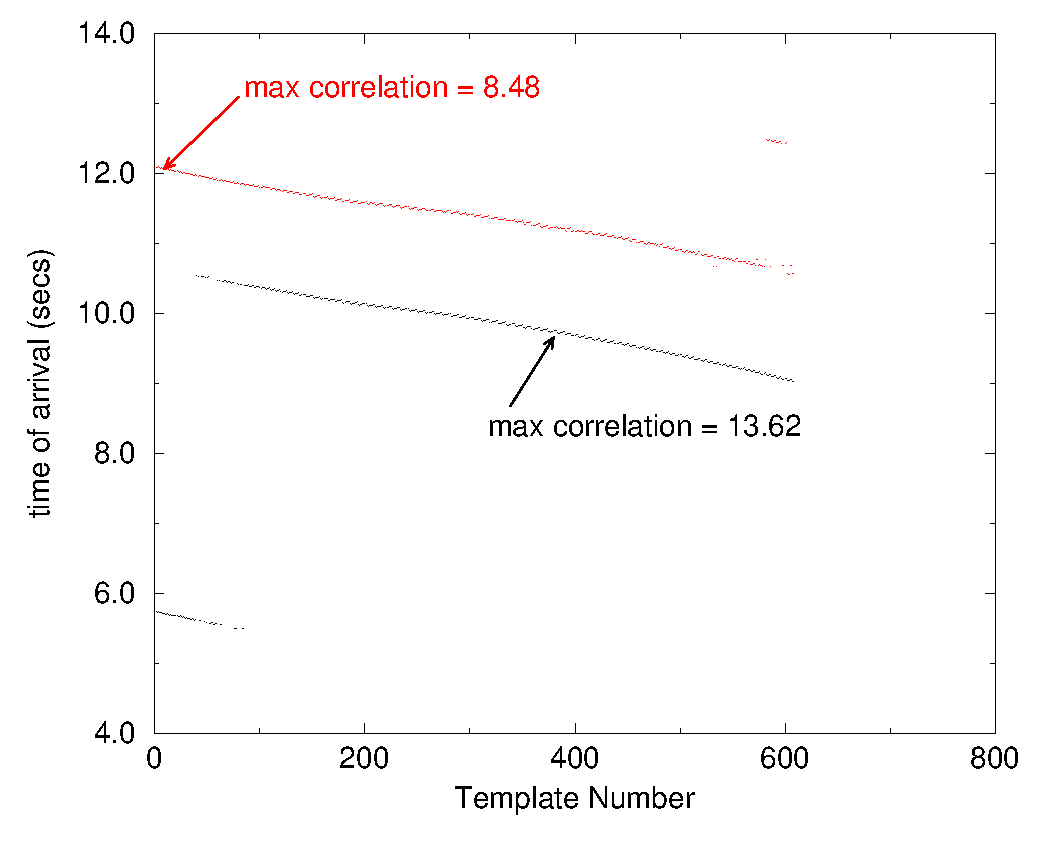
\epsfig{file=Figures/timesofarrival.eps,angle=0,width=4.5in}
\caption{ \label{f:timesofarrival} Variation of time of arrival across template bank.}
\end{center}
\end{figure}
Here again we use the index 0 to denote the first template.
The masses corresponding to the
template number 383 tally well with the those of the 
injected signal (1.4,1.4 solar
mass binary). We observe a well-defined pattern for the $t_a$ across
the template bank.  The templates are roughly arranged in the order of
decreasing masses and consequently of larger chirp times. 
The red points are obtained for segment 33. The maximum SNR obtained
in this case is 8.48. In this segment no chirp signal had been
injected. Again we plot the $t_a$ obtained at various templates.  
The behaviour is remarkably similar to the case where there is
actually a signal present in the detector output. The arrows point to
the template which maximises the correlation. 

A possible explanation for this phenomenon is as follows. Consider
first the case where a signal has been injected into the data (the
black points on the graph).
In this case the template and signal
achieve  a good  correlation if the large amplitudes parts of their
waveforms  are well aligned. In other words the template matches well
with the injected signal if the time of coalescence is the same for
both the template and the injected signal.  
The sum of the chirp times $t_{chirp} = \tau_0+\tau_1+\tau_{1.5}+\tau_2$
is almost equal to the length of the chirp waveform and the
time of coalescence is the sum, $t_C = t_a + t_{chirp}$.
The templates are evenly placed in the $\tau_0,\tau_1$
parameter space and consequently the total chirp time increases
almost linearly with the template number. Since  $t_C$ is being
held constant, $t_a$ must decrease linearly with the
template number. 

Consider now the case when there is no injected signal.
Nevertheless, a large SNR (8.48) has been
obtained. We assume that the high SNR is caused by a
short burst of noise in the data.
The correlation between any template
and a noise burst will be maximised for a time-of-arrival for which
the last few cycles of the template coincide with the noise burst. 
Now since the the chirp times increase roughly linearly as the
template number increases we again have the time of arrival decreasing
linearly.
Thus, we conclude that it is  difficult to distinguish between a correct detection
and a false alarm using this test.

Another possible discriminator could be the variation of the maximum
correlation (maximized over the phase and the arrival times) as a
function of template number. 
In Figure \ref{f:snr-acrosstemplatebank} we plot the maximum SNR
obtained for a template against the template number. The 
black curve represents segment number 2 corresponding to a true
detection and the red curve represents segment number 33 corresponding
to a spurious detection. Again the variation of the SNR with template
number in the two cases does not help in distinguishing a  true
detection from a false alarm.  
\begin{figure}[hb]
\index{colorpage}
\begin{center}
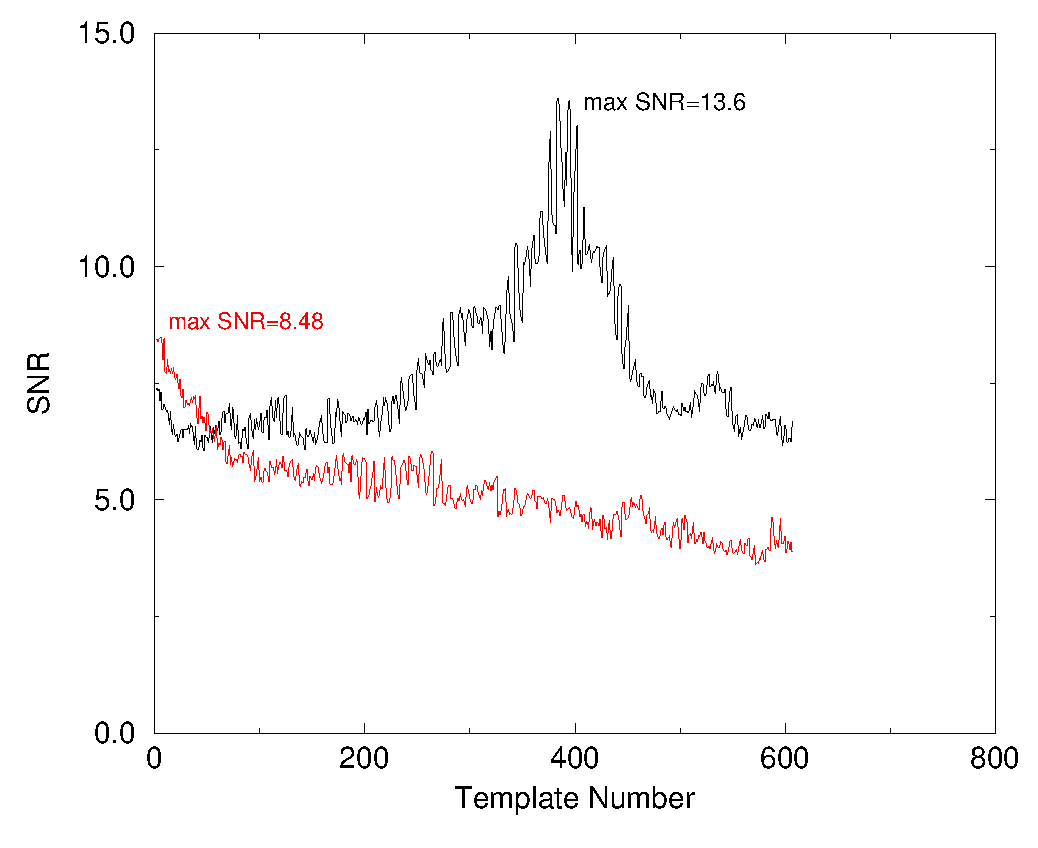
\epsfig{file=Figures/snracrosstemplates.eps,angle=0,width=4.5in}
\caption{ \label{f:snr-acrosstemplatebank} Variation of SNR across the template bank}
\end{center}
\end{figure}



